\documentclass[book.tex]{subfiles}
\begin{document}
\section{Programming}



Development was done with Borland C++ 3.1 (but the language used was C) which by default ran in EGA mode 3 offering a screen 80 characters wide and 25 characters tall.\\
\par
John Carmack took care of the runtime code. John Romero programmed many of the tools (TED5 map editor, IGRAB asset packer, MUSE sound packer). Jason Blochowiak wrote important subsystems of the game (Input manager, Sound manager, User manager).\\

\begin{figure}[H]
\centering
  \fullimage{compiling.png}
\caption{Borland C++ 3.1 editor}
\end{figure}
\par
Borland's solution was an all-in-one package. The IDE, \cw{BC.EXE}, despite some instabilities allowed crude multi-windows code editing with pleasant syntax highlights. The compiler and linker were also part of the package under \cw{BCC.EXE} and \cw{TLINK.EXE}\footnote{Source: Borland C++ 3.1 User Guide.}.
\pagebreak


There was no need to enter command-line mode however. The IDE allowed to create a project, build, run and debug.\\
\par
\begin{figure}[H]
\centering
  \fullimage{borland_compile.png}
  \caption{Compiling Keen Dreams with Borland C++ 3.1}
\end{figure}






Another way to improve screen real estate was to use "high resolution" 50x80 text mode.\\
\par 
 \fullimage{borland_ide_select.png}\\
 \par
 \vspace{-7pt}
The comments still fit perfectly on screen since only the vertical resolution is doubled.\\
\par
\vspace{-4pt}
 \fullimage{borland_ide_highres.png} 
 The file \cw{KD\_MAIN.C} opened in both modes demonstrates the readability/visibility trade-off.\\
\par

  \fullimage{borland_ide_main_lowres.png}\\
\vspace{-5pt}  
   %\vspace{-4pt}
\par
\vspace{5pt}
 \fullimage{borland_ide_main_highres.png}
\section{Graphic Assets}

All graphic assets were produced by Adrian Carmack. All of the work was done with Deluxe Paint (by Brent Iverson, Electronic Arts) and saved in ILBM\footnote{InterLeaved BitMap.} files (Deluxe Paint proprietary format). All assets were hand drawn with a mouse.

\begin{figure}[H]
  \centering
 \fullimage{deluxe_paint.png}
 \caption{Deluxe Paint was used to draw all assets in the game.}
\end{figure}


\section{Assets Workflow}
After the graphic assets were generated, a tool (IGRAB) packed all ILBMs together in an archive and generated a archive header file (\cw{KDR}-format) and C header file with asset IDs. The engine references an asset directly by using these IDs.\\
\begin{figure}[H]
\centering
 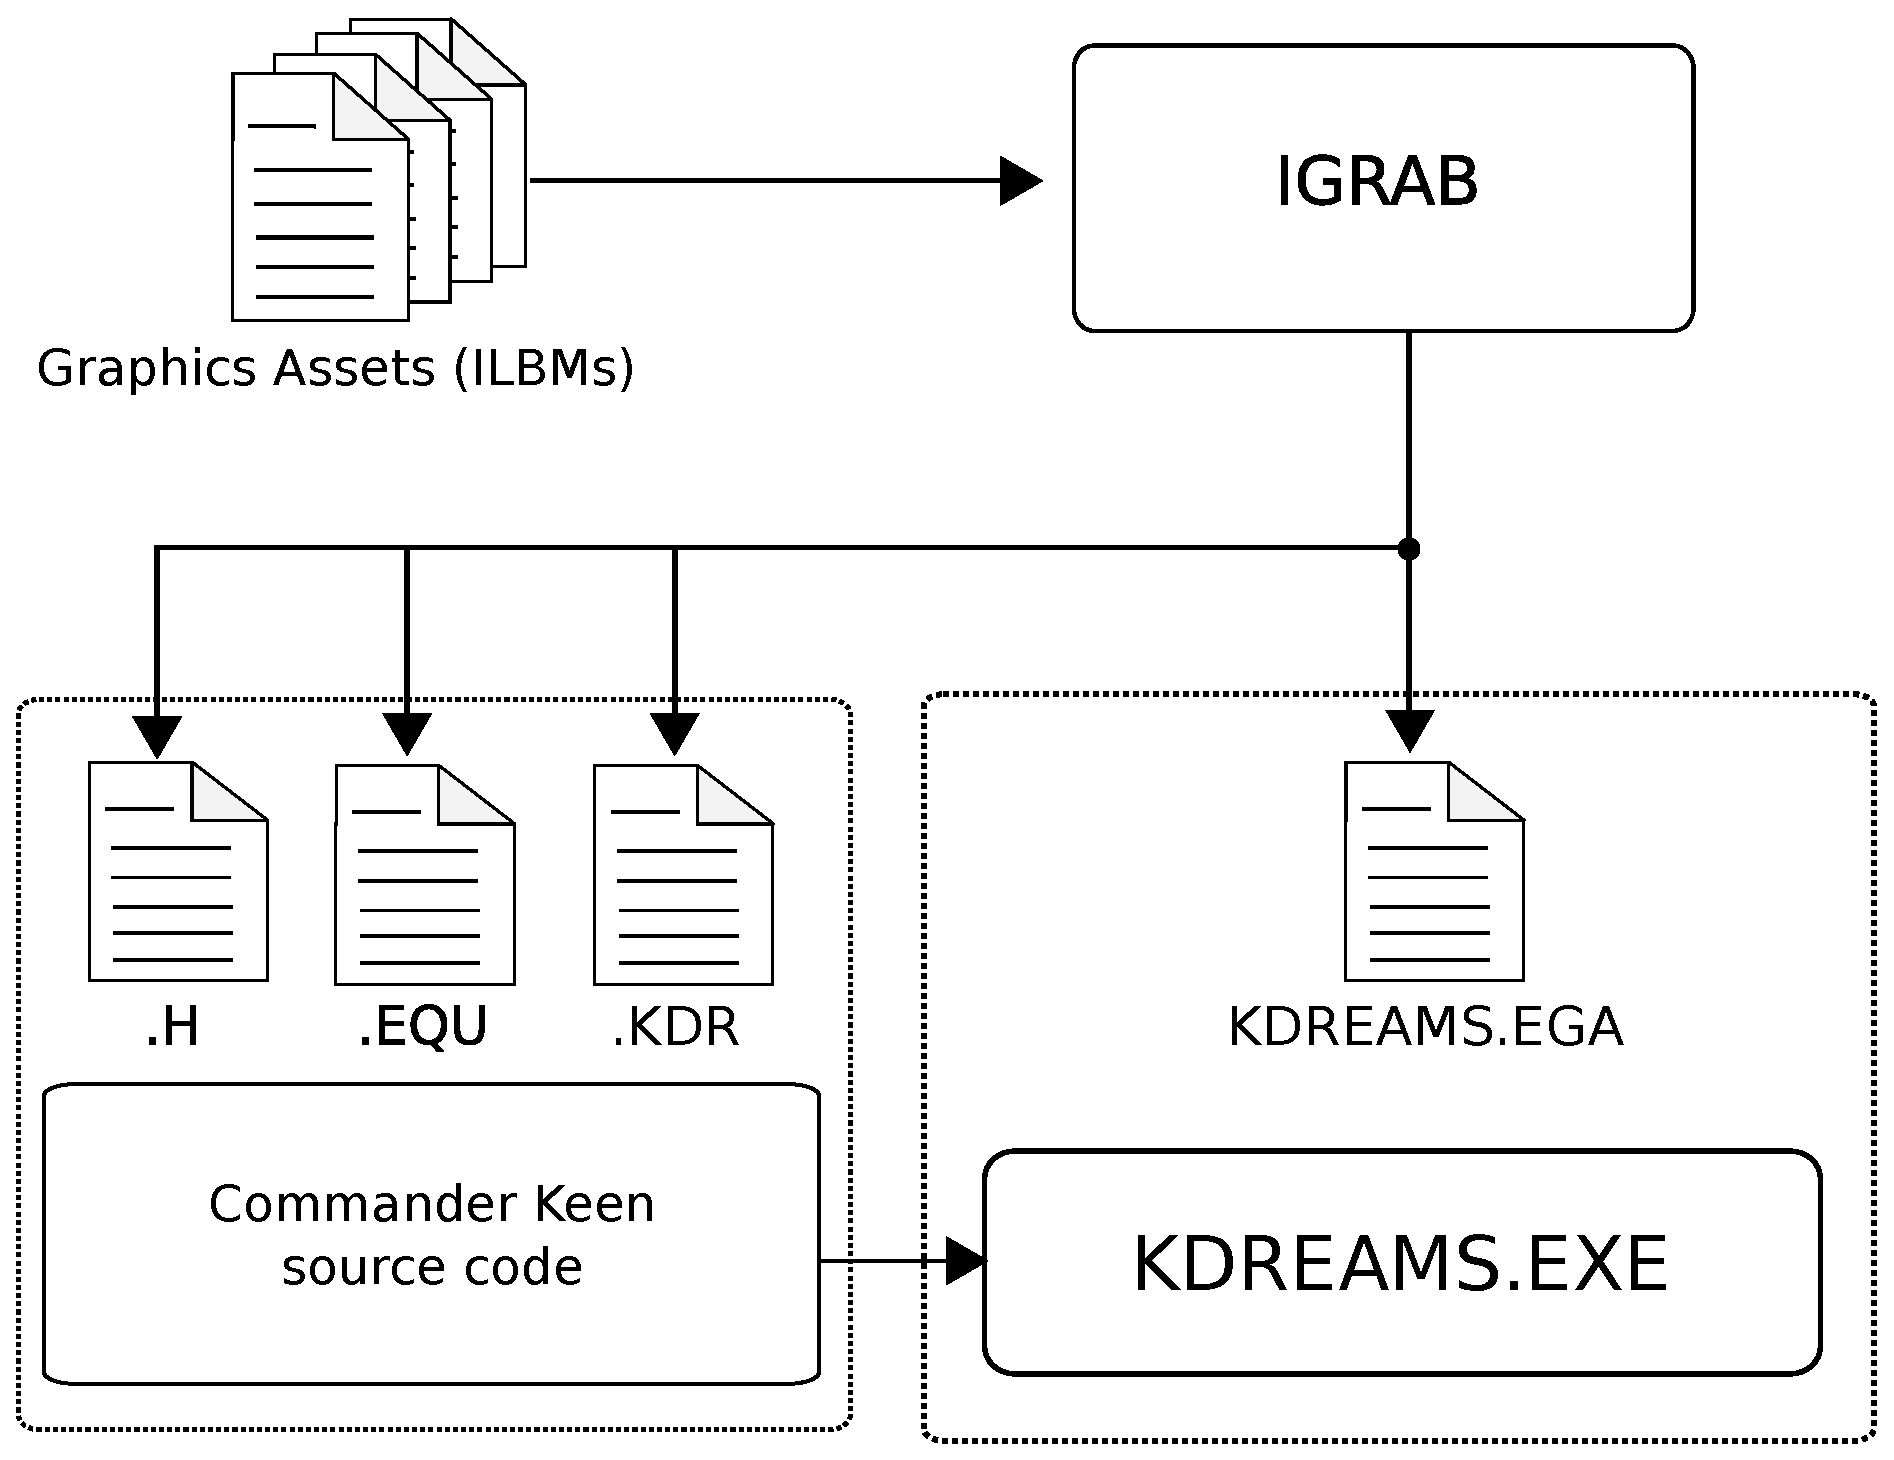
\includegraphics[width=.9\textwidth]{imgs/drawings/drawing_plain.eps}
 \caption{Asset creation pipeline for graphics items}
 \label{asset-creation-pipeline}
\end{figure}
\par
\begin{minipage}{\textwidth}
 \lstinputlisting[language=C]{code/assets_header.c}\par
 \end{minipage}
 
 In the engine code, asset usage is hardcoded via an enum. This enum is an offset into the archive \cw{HEAD} table which gives an offset in the \cw{DATA} archive. The archive header files are stored in the \cw{\textbackslash static} folder.\\

Figure xx shows what is inside the \cw{KDREAMS.EGA} asset file
\begin{figure}[H]
\centering
 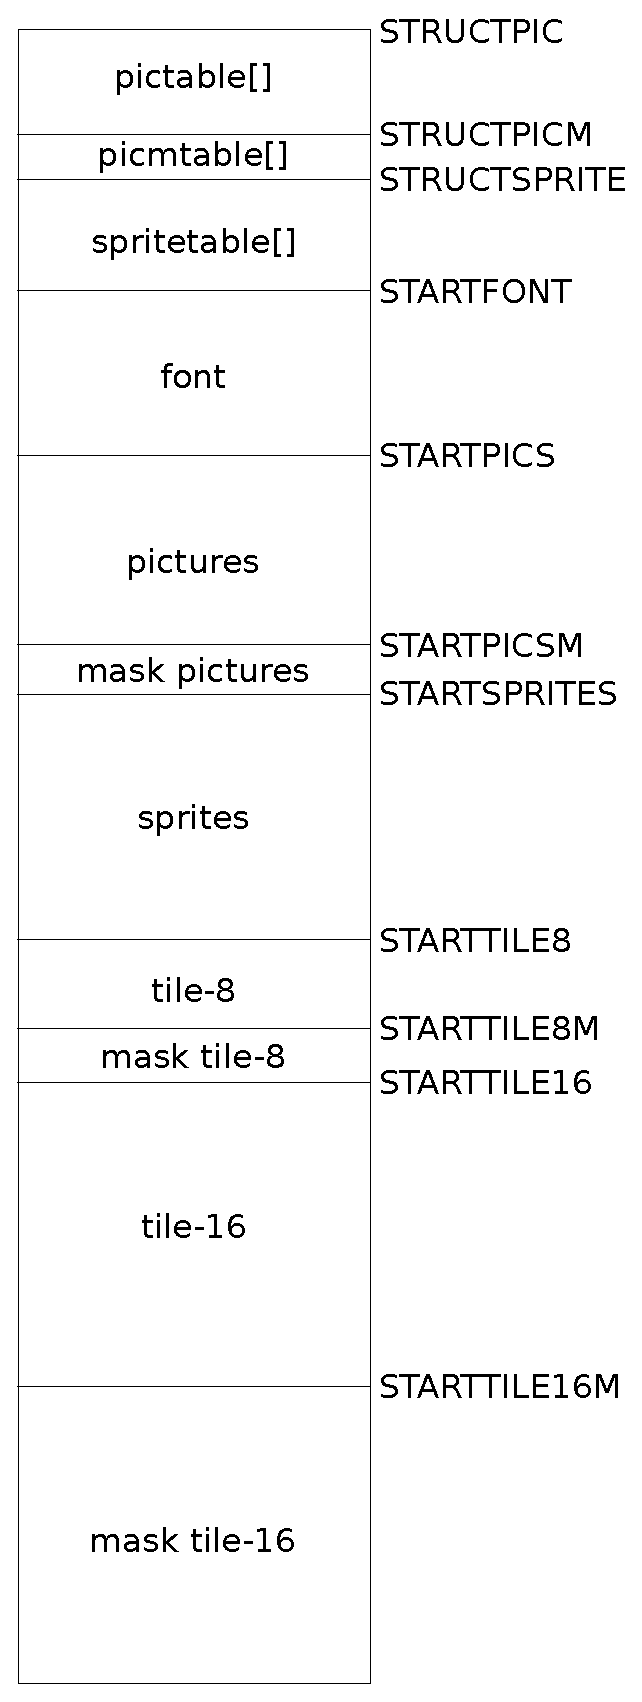
\includegraphics[width=.5\textwidth]{imgs/drawings/graphic_assets.eps}
 \caption{File structure op \cw{KDREAMS.EGA} asset file.}
 \label{asset-creation-pipeline}
\end{figure}

The \cw{pictable[]} contains the width and height for each picture in the asset file. The actual picture data is located in the \cw{pictures} location of the file. The same structure applies for the mask pictures.\\

\begin{figure}[H]
\begin{subfigure}{.5\textwidth}
  \centering
  \begin{table}[H]
  \begin{tabularx}{0.8\textwidth}[c]{lrr}
  \hline
  \textbf{index} & \textbf{width} & \textbf{height}   \\ \hline
  0             & 12          & 13    \\
  0             & 16          & 18    \\

  \end{tabularx}
  \end{table}
  \caption{pictable[].}
  \label{picttable}
\end{subfigure}%
\begin{subfigure}{.5\textwidth}
  \centering
\end{subfigure}
\caption{Tile clipping map}
\label{fig:clip_tinf}
\end{figure}


The \cw{spritetable[]} contains beside width and height also information on the sprite center, boundaries and if a shifted sprite must be created.\\

 

\end{document}
